\chapter{Credit mining implementation and setup}
\label{chp:implexperiment}
In the previous chapter, we discussed the credit mining system design. The system can be implemented in any language with any interpretation of implementation. In this work, credit mining system implemented in Tribler, a python torrent client that was built in Delft University of Technology. Based on this implementation, we come up with the suitable experiment design to answer our research question in previous chapter. 

This chapter consists of the elaboration of both implementation and its experiment execution plan. First, in section \ref{section:triblerintregration}, we will describe how the credit mining system is implemented within Tribler. As Tribler already had a rule for new system that will be integrated, we addressed those rules. We will also look into the challenges that might be faced if Tribler deploy with credit mining system implemented and discuss the possible solution afterwards. After that, we introduce \textit{gumby} on section \ref{section:gumby}, the experiment runner developed by Tribler team in-house. The section \ref{section:cmexp} will follow to explain the actual experiment execution plan. Section \ref{section:cmparamexp} extend those experiments to an extend which it can be configurable in several points.

\section{Tribler integration}
\label{section:triblerintregration}
As a proof of concept, credit mining system was implemented as a module in Tribler. Tribler was built using python, compatible with version 2.x and 3.x. At the time credit mining system implemented in Tribler, Tribler stil use WX as GUI (Graphical User Interface) framework. As for the future, Tribler will move its GUI to use Qt, starting version 7.0 onwards. All of those components made Tribler work cross platform (Linux, MacOS, and Windows).

In the prior work, some of the credit mining system code were implemented by \citeauthor{2015:creditmining:capota} and Egbert Bouman in his Tribler fork\footnote{\url{https://github.com/mihaic/tribler/tree/channel_boosting_new_exp}} instead of the main repository. This made the compatibility and stability between Tribler and credit mining system broke, thus make the system unusable. At this stage, the credit mining code was 1528 line long with 51 deletions.

% implemented in wx for GUI
\subsection{Contribution on software engineering}
As part of the software engineering process, the credit mining code need to be pass several steps before merged into main repository. First and foremost, is to open a Pull Request from forked repository to main. In Tribler, there are two main branch : \texttt{devel} for all new features and fixes, and \texttt{next} which contains bug fixes for the stable release. The pull request of first credit mining prototype was directed to \texttt{devel} branch as it is new feature at that point. Next phase is to work on the code itself by committing the work to the pull request. After that, other member of Tribler will review the implementation. One of the review material is the auto test report that executed by Jenkins\footnote{\url{http://jenkins.tribler.org/}}. The peer review process repeated until no other feedbacks. The lead developer will do a final review afterwards. After they gave OK sign, the commits need to be squashed and finally the pull request can be merged. Figure \ref{fig:cmpullrequest} shows the pull request that has been merged into Tribler main repository on \texttt{devel}.

\begin{figure}[h]
	\centering
	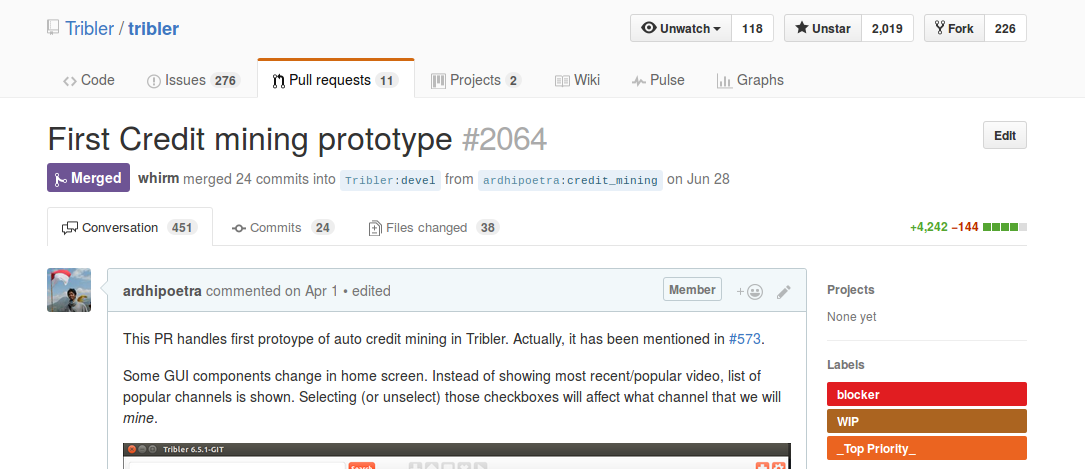
\includegraphics[width=\textwidth]{pics/cm_pr_crop.png}
	\caption[Merged pull request on credit mining prototype]{Merged pull request on credit mining prototype\footnotemark.}
	\label{fig:cmpullrequest}
\end{figure}

As shown in Figure \ref{fig:cmpullrequest}, the first credit mining prototype was heavily discussed by 6 other participants and more than 450 comments. It also takes almost 3 months to accommodate all the feedbacks and reviews. The coverage of this integration worth more than 4200 added lines and 140 deletions. The code portion is quite balanced with 1425 lines goes to GUI part of the code, 1290 lines to the credit mining system itself, 1160 lines to the tests, while the rest to other Tribler components to accommodate credit mining system. At the time of merging, credit mining system passed all the necessary test such and able to run in Linux, MacOS, and Windows (both 32 and 64 bit).

\footnotetext{Available in : \url{https://github.com/Tribler/tribler/pull/2064/}}
\subsection{Experience enhancement}
Credit mining system implementation is made publicly available for end user. It is important to encourage user to be as altruistic as possible. Therefore, in this system, we provide minimal interaction so non-altruistic user can be shown the effect of altruism and be convinced that this behavior is beneficial for both parties. In this part, we will elaborate the effort we have done on enhancing user experience of credit mining system on Tribler. As for comparison, Figure \ref{fig:oldcm} shows the only interface available from the previous work. In this version, it was not possible to add the mining sources except from the Tribler configuration file. 

\begin{figure}[h]
	\centering
	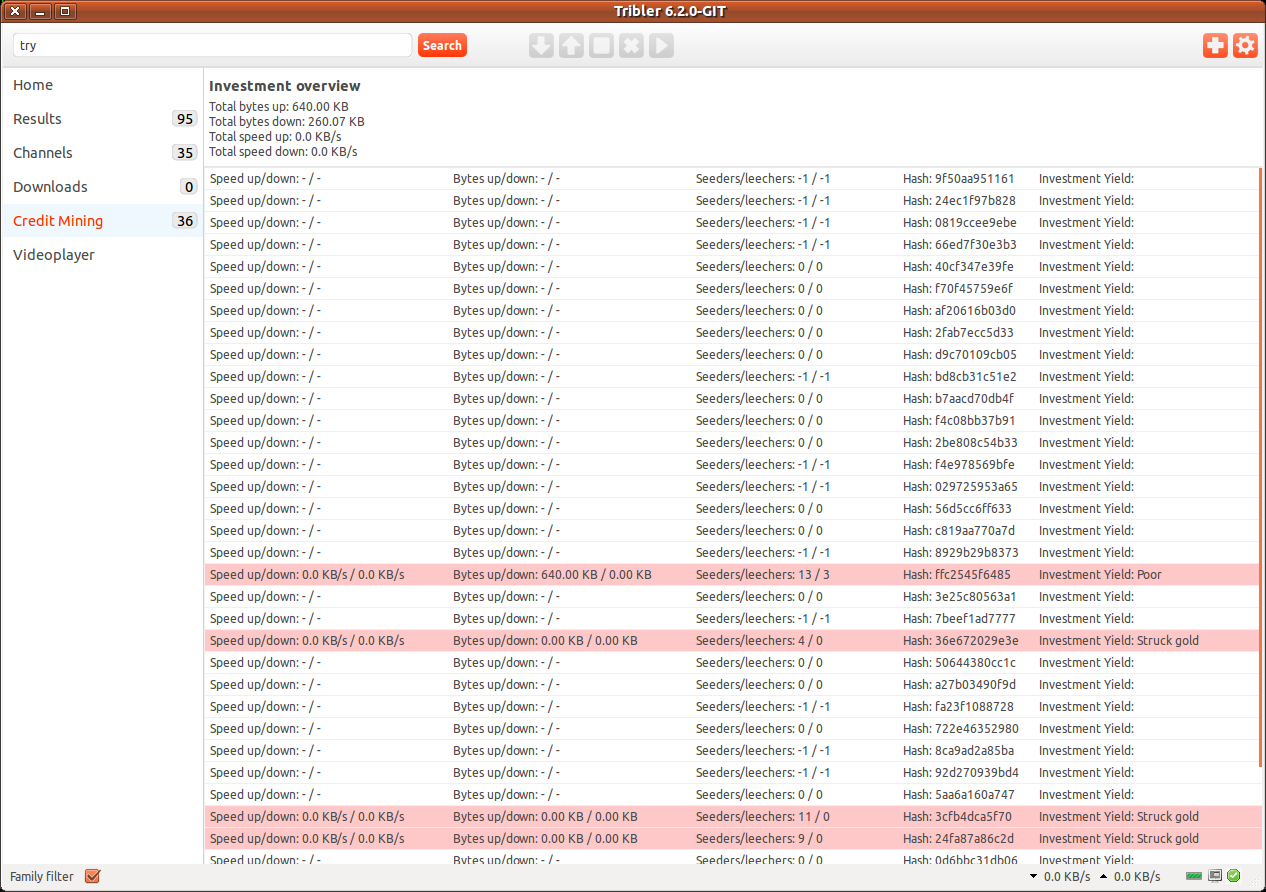
\includegraphics[width=0.8\textwidth]{pics/old_cm.png}
	\caption{The GUI for showing information from prior work \cite{2015:creditmining:capota}.}
	\label{fig:oldcm}
\end{figure}

\subsubsection{Graphical user interface revampment}

Start with the screen we called credit mining main window, it has similar interface compared with previous version. We improved the investment summary by adding more information of the mining source. The investment summary screen contains the swarms download/upload speed, amount of downloaded/uploaded, amount of seeder/leecher, and its identification. Figure \ref{fig:overview} shows this screen. In the same window, we also integrate an interface to easily add or remove mining sources. As mentioned in Section \ref{section:msource}, currently there are only 3 types of sources. Adding RSS and directory source can be done by clicking the upper left option. In the other hand, adding channel source can be done by put the mark in the check boxes in the source list. Figure \ref{fig:addsource} shows the example of adding directory source.

\begin{figure}[t!]
	\begin{adjustwidth}{-2.5cm}{}
		\begin{subfigure}[t]{0.6\textwidth}
			\centering
			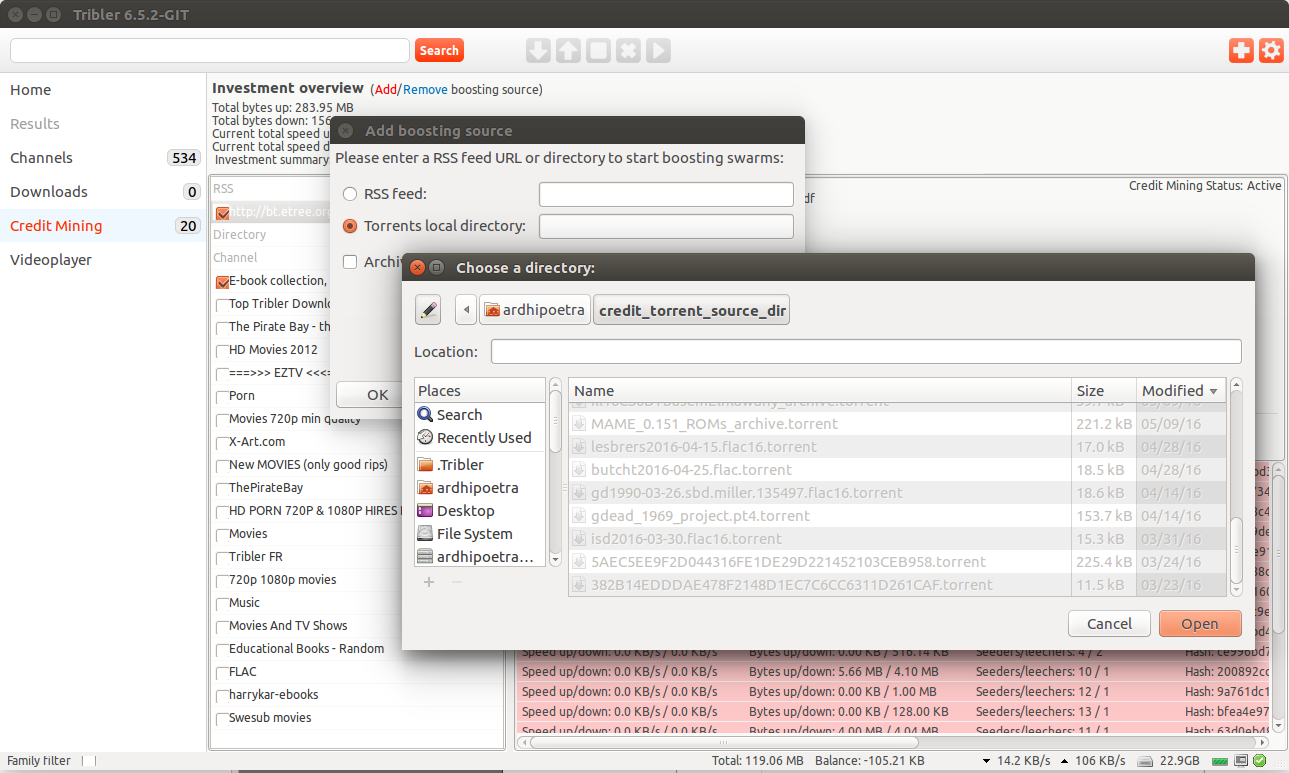
\includegraphics[width=\textwidth, height=6cm]{pics/add_source.png}
			\caption{The interface of adding mining source.}
			\label{fig:addsource}
		\end{subfigure}
		~
		\begin{subfigure}[t]{0.8\textwidth}
			\centering
			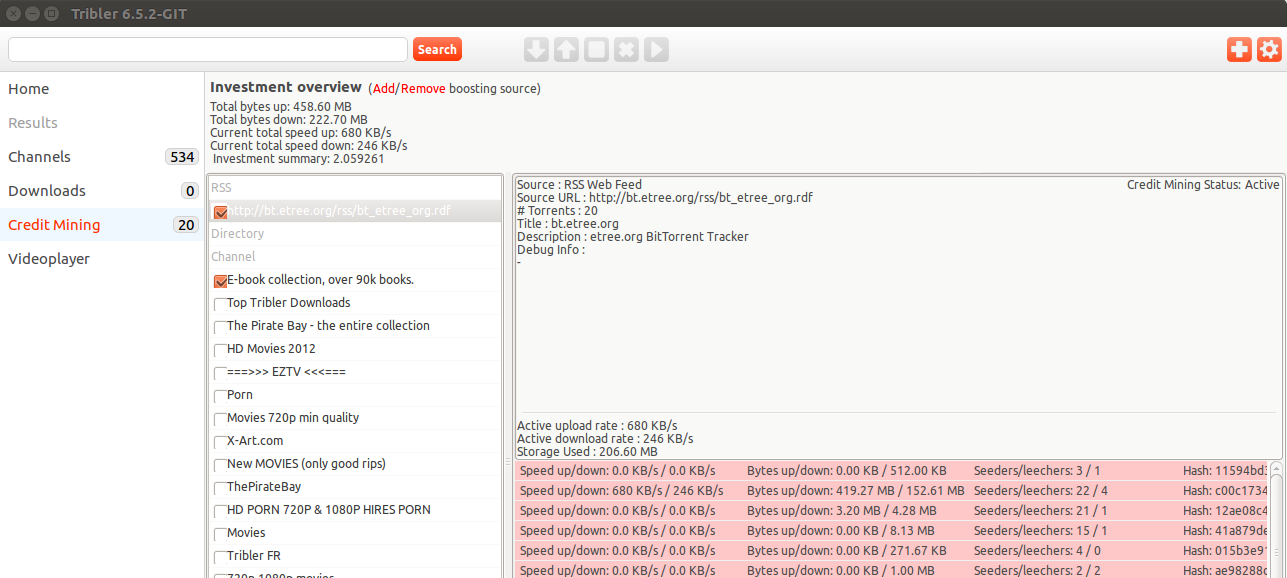
\includegraphics[width=\textwidth, height=6cm]{pics/overview_result.png}
			\caption{The investment overview.}
			\label{fig:overview}
		\end{subfigure}
		\caption{Credit mining main window.}
	\end{adjustwidth}
\end{figure}

Credit mining system is disabled by default in Tribler. Because it relates with automatically upload data, it might be concerned with privacy and security issue on end users. Therefore, a user must opt-in to enable credit mining. It can be done by flag the checkbox in Tribler settings window. After enabled, user need to restart Tribler to have the settings take effect. 

Activating credit mining module made the home screen of Tribler changed. We put several channels sorted by its popularity at the home screen as shown in Figure \ref{fig:homecm}. Channel is an integral part of Tribler which can be used to disseminate swarm information. This way, Tribler user do not need to leave the application to download new content. In home screen, user can simply click which channel he want to mine. This action will also be reflected in the credit mining main screen. To provide user with sufficient information, the popularity, shown by stars in the channel, and the random swarm that resides within that channel is showed. Moreover, user can also look for channel information if necessary. In this way, Tribler user have an easy access to mine a channel, which we strongly recommend.

\begin{figure}
	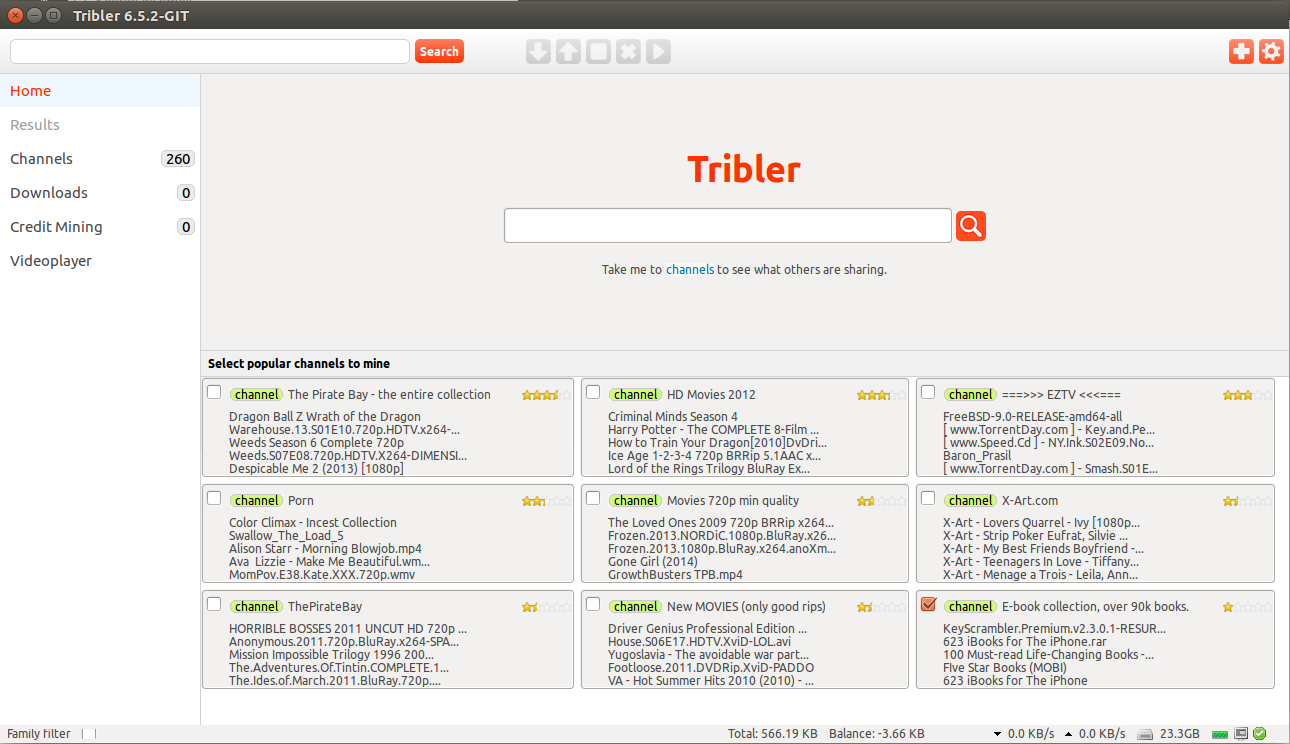
\includegraphics[width=\textwidth]{pics/home_channel.png}
	\caption{The home interface of Tribler with credit mining active.}
	\label{fig:homecm}
\end{figure}

In integrating with Tribler, we emphasize the simplicity to both interact with credit mining system and monitor gained credit. Especially to mine channel, two methods are introduced, both are by single-clicking the checkboxes in home screen (Figure \ref{fig:homecm}) or in credit mining main page (Figure \ref{fig:overview}). Although in the home screen only limited popular channel are shown, in credit mining main page this is not the case. After scrolled some content, if Tribler find another channel that has not been shown, it will append the list with that channel. Basically, it is an infinite list of channel with the upper bound the total number of channel available in Tribler environment. After the channel has been added to credit mining system, user can enable or disable it by another single click.

\subsubsection{User activity awareness}
\label{section:uactivityimpl}
One important point to ensure user to keep using any system is to not disturb their activity. In a typical torrent client, non-altruistic user tend to only activate his client when downloading. Although credit mining system runs automatically, it is possible the system will find a potential swarm then actively download from it. For a user with limited bandwidth, we realize this could be a problem if this user realize his bandwidth that currently used is taken by credit mining system. In a long term, this may cause user to disable this system because of the potential intrusiveness. We define the \textit{user download activity} as the activity that intentionally initiated by user in order to participate or download content on the particular swarm. Usually, it is the true purpose of having torrent client. 

\todo{Restructure the following}In response to that issue, on the integration with Tribler, we also implemented another module in credit mining system to adjust its mining activity to user download activity. Credit mining system periodically check whether there is an user downloading activity. If there is not any, then credit mining system can notify the miners to use all the bandwidth available. If there is an activity, user need to set the priority of credit mining download activity. By default, the priority of credit mining download activity will be reduced to one-third\todo{tentative : one-third/3 times}. This means, the swarm in the user download activity will get 3 times higher probability of bandwidth allocation compared to the one in credit mining download activity. The bandwidth distribution is not strictly in order, however, the priority is used as weight for it.

%\subsubsection{Libtorrent tuning}
%settings in libtorrent to accommodate credit mining <- removed it for now.

%\subsection{Anonymous and secure mining}
%\todo[inline]{untested. May skip this subsection. See .tex file for draft}
%Tribler is well known for its anonymity and secure interface on top of \bt~ network. In 2014, Tribler published a specification on its anonymity feature\footnote{\url{https://github.com/Tribler/tribler/wiki/Anonymous-Downloading-and-Streaming-specifications}}. It uses Tor-like onion routing with purely distributed mechanism. A year later, \citeauthor{2015:tunnel:ruigrok} on his work completed the \textit{tunnel community} which emphasize end-to-end encryption in Tribler. This comes with several drawbacks. The most important one is performance degradation. Adding layers of privacy comes with increasing the amount of cryptography operation which slows down end-to-end downloading activity \cite{2015:tunnel:ruigrok}.

% enable safe_seeding: when finished and in 'seeding' state. hops: download/upload via libtorrent proxy.

\section{Gumby}
\label{section:gumby}
After credit mining system is integrated with Tribler, the next part is to test whether the implementation showing expected result or not. One way to conduct the experiment is by launching Tribler clients in the wild and monitor them using reporting mechanism. Another method is by create several virtual machines and launch Tribler within it. Both approaches are not scalable and very difficult to automatize. Fortunately, in Tribler, there is an experiment runner that can be used to run Tribler in both local machine or cluster to emulate the experiment.

\textit{Gumby}\footnote{\url{https://github.com/Tribler/gumby}} is an experiment runner framework for performing in both Tribler and Dispersy. Gumby can run both in local computer and cluster computer. In this case, we able to run gumby in DAS4 and DAS5 (via Jenkins) as part of our experiment. Gumby run on different scenarios that can be specified. It uses configuration file for each experiment to define all the settings needed for one run. Developer can easily specify the number of peer needed for one experiment, the post process script after running experiment, the value that needed to be distributed to all of the peers, and many others. The most important part is to code the experiment code itself written in \texttt{python}. In this file, one must define how the experiment will run and behave. How the commands interpreted also described in this file. There are some functions and classes that need to be extended to make the experiment works.

Gumby run in sequential manner with several steps. The set of steps are different depends on the flag specified in the configuration. But in general, the run is executed as follows. First, gumby read the scenario and configuration file. After deciding what type of experiment it has to run, it will clear the output directory and synchronize it on multiple nodes, in case of running it in cluster computing. Next, the setup script will be executed. It usually contains the experiment requirement that need to be built. After that, it spawns Dispersy and experiment tracker to monitor the experiment in case of error occurred. All of the experiment nodes communicate with server using specified IP and port. Server also expected to exchange messages between nodes whenever needed or specified in the scenario. Finally, both local and remote processes are started in parallel. Upon finishing experiment, server will wait all node instances to exit and disconnect. Then it will copy the data to predefined directory which can be processed using specified post-experiment script to generate items such as graphs and tables.

\subsection{Scenario and Configuration}
In gumby, it is not possible to intervene the experiment on the fly. What the developer can do is by specifying commands in scenario file. The scenario notation is quite simple. It only needs the time of an action that has to be executed and the command itself. Optionally, which node that run the command can also be specified. Figure \ref{fig:gumbyscenario} shows the example of the aforementioned scenario. For example, command \texttt{@0:36 set\_boost\_settings boosting.ini.1 \{3\}} means in seconds 36, gumby will run command \texttt{set\_boost\_settings} with \texttt{boosting.ini.1} as parameter on node number 3. 

\begin{verbbox}
@0:0 set_master_member 3081a73010...e75
@0:2 start_dispersy {1-3}
@0:10 start_session
@0:22 online
@0:23 set_speed 0 0 {3}
@0:32 create {1}
@0:35 publish file1gb_1 1524288077 {1}
@0:36 set_boost_settings boosting.ini.1 {3}
@0:37 start_boosting {3}
@0:40 add_source http://bt.etree.org/rss/bt_etree_org.rdf {3}
@1:15 start_download file1gb_1 {2}
@1:33 reset_dispersy_statistics
@0:43100 stop
\end{verbbox}

\begin{figure}[h]
	\fbox{\theverbbox}
	\caption{Scenario format example}
	\label{fig:gumbyscenario}
\end{figure}

With scenario defined as a custom format, on the other hand, gumby configuration file only contains the number of variables that need to be filled. These variables can be accessed from inside the program. Figure \ref{fig:gumbyconf} shows the example of configuration format in gumby. There are some necessary variables such as experiment name and \texttt{tracker\_cmd}. Some of the variables required by specific conditions. For example, if \texttt{local\_instance\_cmd} is \texttt{'das4\_reserve\_and\_run.sh'}, it is necessary to call the other 4 subvariables that recognized by \texttt{das4\_} precedence. Lastly, there are variables that completely optional or needed by the experiment file. In this case, specifying \texttt{scenario\_file} is optional to direct whith scenario we want to run in a single experiment.

\begin{verbbox}
experiment_name = "CreditRunner_base_DAS"
experiment_server_cmd = 'experiment_server.py'

local_setup_cmd = 'das4_setup.sh'
local_instance_cmd = 'das4_reserve_and_run.sh'

output_dir = '/var/scratch/aputra/cmining'

das4_node_amount = 2
das4_node_timeout = 3600
das4_instances_to_run = 5
das4_node_command = "creditmining.py"

tracker_cmd = 'run_tracker.sh'

use_local_venv = True

scenario_file = "creditmining_base.scenario"
post_process_cmd = "gumby/scripts/post_credit_mining.sh"
\end{verbbox}
\begin{figure}[]
	\fbox{\theverbbox}
	\caption{Configuration format example}
	\label{fig:gumbyconf}
\end{figure}

\section{Experimental setup}
\label{section:cmexp}
We now focus on how the credit mining system will be evaluated by its performance. In general, there are two aspects we want to address. First one is how credit mining system can gain benefit to its user. This means a user is expected to get considerable amount of credit with small investment. The parameter for this experiment can be derived from how much user actually gain and how it compares to the investment they already had. Second perspective is finding out how the credit mining system can benefit the swarms as a whole. It can be done by monitoring the performance of each of the peers. If each of the peers performance are increasing, then the swarm itself have its capacity increased as well.

\subsection{Experiment conditioning}
The experiments were conducted in different scenario and architecture. For RSS source, we used etree.org (\url{http://bt.etree.org/rss/bt_etree_org.rdf}) and our custom RSS feed. We launced our RSS feed in \url{https://rss-creditmining.herokuapp.com/feeds/}. We put different kinds of swarm there from old but popular to recent but very few peers. Etree.org is a legal community that shares music with permission from authors. This community is relatively active and new published swarm usually has sufficient supply and demand for testing. In the custom RSS feed, we also publish the swarm in different period\todo{Do this}. This approach is important to limit the choice available for credit mining system either from prior or this work. \todo{jenkins, DAS, specification}

Beside putting the credit mining system in the wild, we also conducted an experiment where we can directly observe the swarm. This can be done in gumby by specifying a number of nodes, mechanism of swarm dissemination, and each of the node's activity. We created a swarm with dummy files as a content. This swarm then inserted into a particular \textit{Channel}. This \textit{channel} can be accessed from all the nodes using Dispersy. In the end, user can only get the metadata of this swarm such as files information, infohash, and other thing typically found in \texttt{.torrent} file. 

In our controlled environment, a node can be categorized as publisher, seeder, downloader, or credit miner. A single node will act as a \textit{publisher} of this swarm. It creates \textit{channel} and dummy files, generates metadata, pushes it into the \textit{channel}, and seed for the rest of the experiment. Another node can help become a seed for the swarm if necessary. It need to copy files related to that swarm into their own directory via unthrottled connection. For other node, it can be either download or activate credit mining system. This \textit{channel} can be added to credit mining system as a mining source. As for downloaders, they can both start and stop downloading from a swarm identified by its name. 

\subsection{Comparing performance with prior work}
One checkpoint of this work is comparing the performance to prior work. In the prior work by \citeauthor{2015:creditmining:capota}, they used \textit{net upload gain} as a parameter to measure how many credit user already gain. Net upload gain is a difference between uploaded and downloaded bytes. Moreover, to measure the efficiency of credit mining system, they also defined \textit{normalized upload gain} which is the ratio between \textit{net upload gain} and total downloaded bytes. As an extension of this metric. \todo{add more metrics for comparison}

The comparison experiment will be run for 12 and 24 hours\todo{may change}. As a note, prior work run its experiment for 2 days (48 hours) straight. Etree.org will be used as mining source because other sources are not compatible with the prior work. It is also not compatible with our experiment framework, gumby, to test in closed environment. The recommended parameter on prior work is by setting credit mining system with SeederRatio policy, target ratio 3, and 5 minute swarm interval although in their argument, setting target ratio as 1 gives higher net upload gain. In our experiment, we will use the same parameter and configuration. We will use this performance of credit mining system as \textit{base performance}. It will then referred from other experiment result. 

The problem with running in the wild is the result may different for each time it was run. If we run the program in parallel, there is a possibility that it will intervene each other. Therefore, we will run the experiment in the following method. First, the experiment will be executed one after another. Our experiment will start first. Then, after it finished, the experiment from prior work will be run immediately. We run the program for 12 hours for both, and then for 24 hours after both of them finished. After all the execution completed, we will run both versions in parallel to find out if it intervenes one another. This phase will run for 12 and 24 hours. If necessary, the experiment will be run several times\todo{may change}. Two approach of interpreting the different results will be applied. First approach is ,we will count the average of the results. Other approach is to see the general trend of the result and pick up the majority as sample. 

\subsubsection{New policy}
%run same experiment as above but change the seeder ratio with scoring ratio. 
After knowing the base performance of credit mining system, it is important to keep extending it. By the introduction of our new policy, scoring policy, we intend to compare it to the base performance. In this aspect, we will run two experiment. The first one is the same as previous experiment of etree.org but only change the policy and its parameters. It will be run for both 12 and 24 hours. The result of this experiment will be compared to both prior work and base experiment. 

%run in closed environment. Compare with other policy.
%The second experiment is executed in closed environment. We will observe both local gain of the miners and global benefit that occurred on the swarm. 

\subsection{Predownload hit capabilities}
Credit mining system has many limitations that comes from both resource and libtorrent limitation. Therefore, given a large number of swarms, it is impossible to mine all of them and get good results. Instead, credit mining system measure the swarm before start mining by \textit{predownloading}. However, not all the swarms in the Internet available for predownload. Some swarms are not complete (no one has complete files), only have \textit{webseeds}, and have invalid or duplicate content. This experiment will show how is the prospect of \textit{predownload} in the Internet on a large scale. 
This experiment to check how is the availability torrent in the net.

In this experiment, we only focused on the \textit{predownload} phase. Therefore, it is tailored to not continue mining with the purpose of accommodating a large amount of swarm we intend to process. Because of this flexibility, we increase the maximum swarm per source by hundredfold and set the active swarm to zero. We comply with the default \textit{predownload} default settings in this experiment. After a swarm has been predownloaded, instead of send it to miners, we retrieve the information and then delete it afterwards. By this approach, the swarm per source slot will be freed faster. 

Still, there is limited time for a swarm to be finished. If the time needed for predownloading is more than 1 hour, we mark it as timeout. In fact, the system will not wait until it finished. It will stop when reaching 1 hour period. If the swarm has not finished until the experiment is finished, then it will be marked as unfinished. This is the case where the predownload activity for that swarm just started in less than 1 hour before experiment finish. Maximum number of swarm in a source also contributing to predownload time. The larger the number, there are more active connection and memory needed for storing the data in a single time. In a sense, it might be possible to affect all of those swarm and make it slower to finish the predownload.

%Current ready : 42 Download only 4 pieces. How long it takes.

After a swarm has been predownloaded, we also observe the peer that has discovered. We put two checkpoints of peer discovery. First is when the swarm just finished predownloading. This is the number of peer that discovered along with the predownloading. Second is after waiting period. This period is designed as a time to gather more information of the swarm. A peer as a Web seed or http seed are excluded from the list. It is possible that there are only some peers in a swarm with finished predownload, but the peer discovered is empty. By doing this, we intend to evaluate the overall predownload period and its timing mechanism. \todo{temp:how many peers discovered}

\subsubsection{Torrent crawler}
For this experiment to be succeed, the large number of swarms needed. Although this can be retrieved from anywhere including illegal swarm, we want to contribute to the society by providing support for the legal one. We implemented legal torrent crawler that can be accessed in \url{https://github.com/ardhipoetra/legal-torrent-crawler}. It uses \textit{scrapy}\footnote{\url{https://scrapy.org/}} as a scraper for the torrent portal sites. The crawler will access those sites, find any link to \texttt{.torrent} file, then download and categorize it. So far, we has implemented for 8 sites as shown in Table \ref{tbl:legaltorrentsource}.

\begin{table}[h]
	\centering
	\caption{Legal torrent source.}
	\label{tbl:legaltorrentsource}
	\begin{tabular}{lp{9cm}}
		\hline
		Source & Description \\ \hline
		\url{etree.org} & Live music trading community. \\
		\url{legittorrents.info} & Self-moderated torrent tracker and portal. \\
		\url{librivox.org} & Public domain audiobooks read by volunteers. \\
		\url{linuxtracker.org} & Linux distro torrent aggregator. \\
		\url{distrowatch.com} & Linux distro torrent aggregator. \\
		\url{mininova.org} & Torrent directory site. Used to host copyrighted material but now is no more.\\
		\url{sxswtorrent.com} & Sample music sharing on SXSW events. \\
		\url{vodo.net} & Media distributor that offers legal films, books, games and music.

	\end{tabular}
\end{table}

The crawler is completely unrelated from credit mining system. It can be executed independently. We first executed the crawler first to collect \texttt{.torrent} file and then put it into one directory. After that, the predownload hit experiment is performed.

\subsection{Experiment on user activity}
As mentioned in \ref{section:uactivityimpl}, credit mining system that implemented within Tribler need to accommodate user download activity when mining. This experiment validate that feature by evaluating that there is insignificant effect for user. The expectation is that when both credit mining and user download active, the bandwidth used in user download will keep stable. If only credit mining is active, then it will maximize the bandwidth if possible. For the base data as comparison, the download speed without activating credit mining will be averaged.

The experiment will start in closed environment with 10 nodes. In the scenario, we defined three swarms that available for download. As for node categorization, single node act as a publisher, 7 nodes as seeder, the rest are downloaders. One of the downloader activating credit mining and adding our custom RSS feed as its source. We designed the RSS feed that it will feed relatively popular swarm that easy to mine. The download activity will be started first. Credit mining system will be started in several minutes after that. In the middle of scenario, the downloader stop to download one swarm and then switch to another swarm. We will then compare the download speed of one with credit mining active and one without. 

%The Latest try : 42. 
%Make all credit mining priority as 1 if there is a main activity. Commented out peer logging (reduce size)

\section{Finding best parameters}
\label{section:cmparamexp}
The challenge of designing a configurable system is to know what is the effect of the parameters on its performance. Although in the implementation there are many parameters such as the checking period, blacklist threshold and its recovery time, and number of concurrent active swarm in miners, we focused on one that directly related to prospecting method. Therefore, we ended up with two key parameters that need to be evaluated : scoring policy multiplier and the number of downloaded piece in predownload phase.

The experiments in this category will be conducted in both closed environment and the net. In closed environment, we will compare the properties of the swarm observed. The comparison with base performance where credit mining system is not deployed is performed. On the other hand, when launching in the net, custom RSS feed is used. In this case, our focus will be how the credit mining system gain the credit with provided configuration. Both types of experiment run in DAS 4 for 6 hours with 120 nodes. 

\subsection{Multiplier in scoring policy}
We have mentioned scoring policy in section \ref{section:prospection}. It works by considering swarm properties then gives a score for the properties. There is a weight/multiplier for each properties that stands for its importance. In this experiment we change the multiplier to find out which property and what weight best represent the swarm for prospecting purpose.

We choose the minimum and maximum multiplier by 1 and 5, respectively. In this experiment, a properties is prioritized when the multiplier is 5. On ther other hand, it is not prioritized when the multiplier is 1. Considering there are three properties that need the multiplier, there are six combinations of prioritizing the properties. The algorithm will be executed for every 1 hour. We take note the swarm it choose and compare it to base experiment. The more swarms that selected correctly, the better multiplier combination define the swarm.

\subsection{Number of piece download}
Another important point of credit mining system is \textit{predownload} phase. By downloading several pieces in start, we put a capital investment hoping that it will act as a mining catalyst. Intuitively, the more capital investment is placed, the higher return will be gained. However, this is not the case in short or medium period. Moreover, another point of \textit{predownload} also to observe peers to get swarm information. Put a large investment on front may become obsolete in next several round.

We start by disabling the predownload, that is, by set zero as number of piece that need to be predownloaded. Next is by set the number as 4, 20, and 50 to represent few, medium, and many piece, respectively. The number of peer and consumed storage are observed. Then, the chosen swarm that relies on the information generated by \textit{predownload} is noted. To have relatively stable number of peer, we will use custom RSS feed to provide us with old but popular content. 
%\subsection{Peer translation accuracy}

\newpage
\section{Summary -delete me-}
\begin{itemize}
	\item etree RSS: new (seeder ratio) vs mihai's \\
	12 and 24 hour. Each several times. Net upload gain, share ratio.
	\item etree RSS: new (scoring policy) vs mihai's\\
	12 and 24 hour. Net upload gain, share ratio.
	\item predownload hit\\
	pie chart (percentage), histogram (time). For peers :histogram (\# peer), pie (just finished \% of end of measurement)
	\item user activity\\
	speed graph (x-time, y-speed, line-infohashes). Compare with and without credit mining.
	\item changing multiplier\\
	6 experiments. each 6x2=48h
	\item changing piece predownload\\
	0,4,20,50. 6h local. 6h old but popular swarm.
\end{itemize}
